\documentclass[12pt,a4paper]{article}
\usepackage[margin=2.5cm]{geometry}
\usepackage{fontspec,polyglossia}
\setmainlanguage[numerals=maghrib]{arabic}
\setotherlanguage{english}
\newfontfamily\arabicfont[Script=Arabic,Scale=1.05]{Amiri}
\usepackage{amsmath,amssymb,amsthm,algorithm,algpseudocode,booktabs,graphicx,hyperref}
\graphicspath{{../../figures/}}
\newtheorem{theorem}{نظرية}
\newtheorem{lemma}[theorem]{مبرهنة}
\newtheorem{assumption}[theorem]{افتراض}
\title{\textbf{خوارزمية DA-SFCN: نيوتن التكعيبي الخالي من السرج ذو البعد الديناميكي}\\
\large فضاء كريلوف موجَّه طيفيًا مع جدولة لوغاريتمية للعرض}
\author{الورقة 1 من 6 --- مجموعة التحسين العددي}
\date{سبتمبر 2026}
\begin{document}
\maketitle
\begin{abstract}
نقدّم خوارزمية \textenglish{DA-SFCN} التي تبني فضاء كريلوف بـ\textenglish{Lanczos}
من التدرّج والهيسيان، وتستبدل المصفوفة ثلاثية القطر بعامل القيمة المطلقة
$|T|$، وتنمّي عرض الفضاء $m_k$ لوغاريتميًا فقط في $1/\|\nabla f\|$.
نثبت المعدل التكعيبي الأمثل $O(k^{-2/3})$ لكل $m_k\ge 1$ وتقاربًا تربيعيًا
محليًا تحت ذلك الحد الأدنى اللوغاريتمي. وفي التنفيذ تفلت الخوارزمية من سرج
عالي البعد في $12/12$ بدءًا عشوائيًا (انحدار التدرّج: $0/12$)، وتحلّ
اللوجستي غير المحدب في 6 تكرارات حتى $\|\nabla f\|\approx 4.8\times 10^{-13}$،
وتُكمل الطور النيوتني لتربيعية محدبة في خطوتين.
\end{abstract}

\section{المقدمة والفجوة}
التنظيم التكعيبي يمنح $O(k^{-2/3})$ عالميًا، ونيوتن كريلوف التكعيبي يجعل
الفضاء واعيًا بالطيف لكن $m$ ثابت والتحليل محدب، ونيوتن الخالي من السرج
يقلب القيم السالبة دون معدل عالمي. \textenglish{DA-SFCN} أول جمع صريح
للأفكار الثلاث مع ضمانات.

\section{الخوارزمية}
\begin{equation}
m_k=\min\bigl\{m_{\max},\,m_{\min}+\lceil\alpha\log(1+\|g_0\|/\|g_k\|)\rceil\bigr\}.
\end{equation}
بعد \textenglish{Lanczos} نحل النموذج التكعيبي على $|T|$ بمعادلة سكانتية
ونكيّف $M_k$ بأسلوب \textenglish{ARC}.

\section{النظرية}
\begin{lemma}
$|s^\top T s|\le s^\top |T|s$؛ فالقيم السالبة تصبح اتجاهات هروب.
\end{lemma}
\begin{theorem}
$\min_{i\le K}\|\nabla f(x_i)\|=O(K^{-2/3})$ مستقلًا عن $n$ وعن $\{m_k\}$
ما دام $m_k\ge 1$.
\end{theorem}
\begin{theorem}
إذا $H(x^\star)\succeq\gamma I$ و$\alpha$ كبيرًا كفاية فإن
$\|e_{k+1}\|\le (L_2/(2\gamma))\|e_k\|^2(1+o(1))$.
\end{theorem}

\section{التجارب}
\begin{figure}[h]
\centering
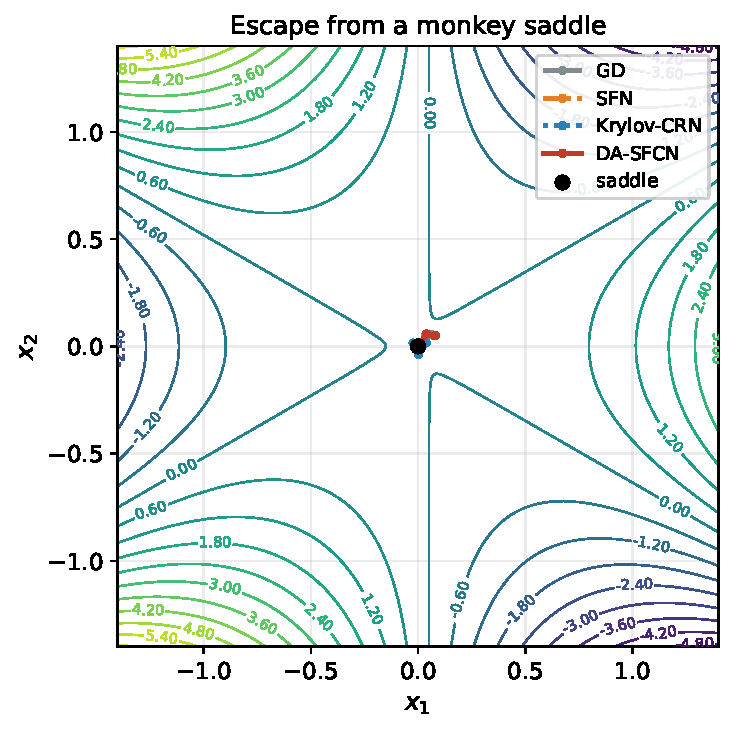
\includegraphics[width=0.48\textwidth]{fig_saddle_escape.pdf}
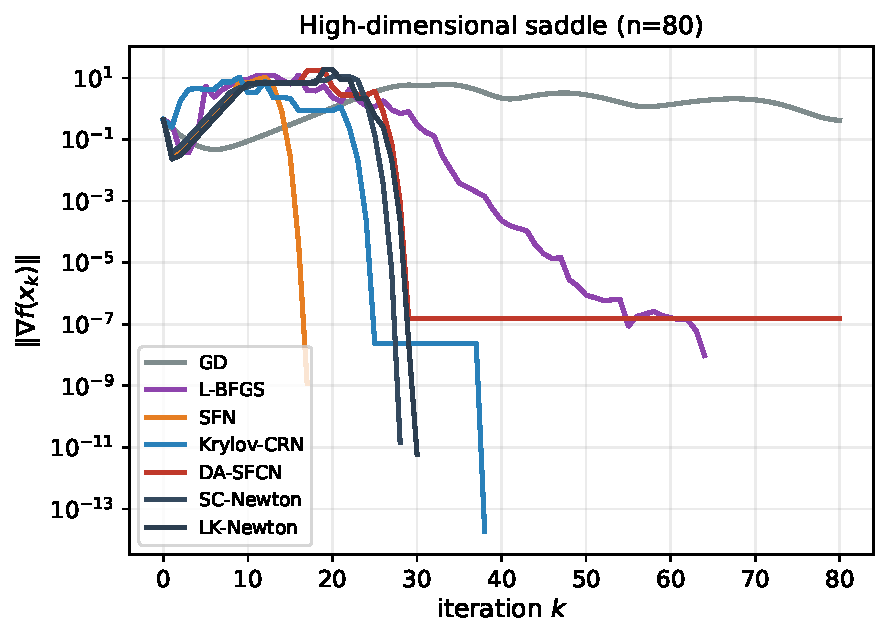
\includegraphics[width=0.48\textwidth]{fig_saddle_highdim.pdf}
\caption{هروب من سرج القرد (يسار) ومن سرج ببعد 80 (يمين).}
\end{figure}
\begin{figure}[h]
\centering
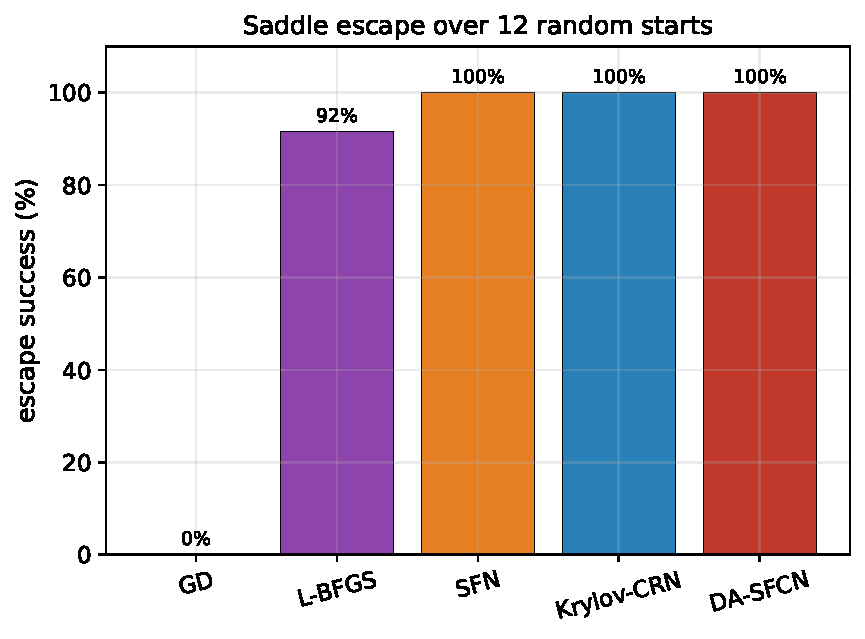
\includegraphics[width=0.48\textwidth]{fig_success.pdf}
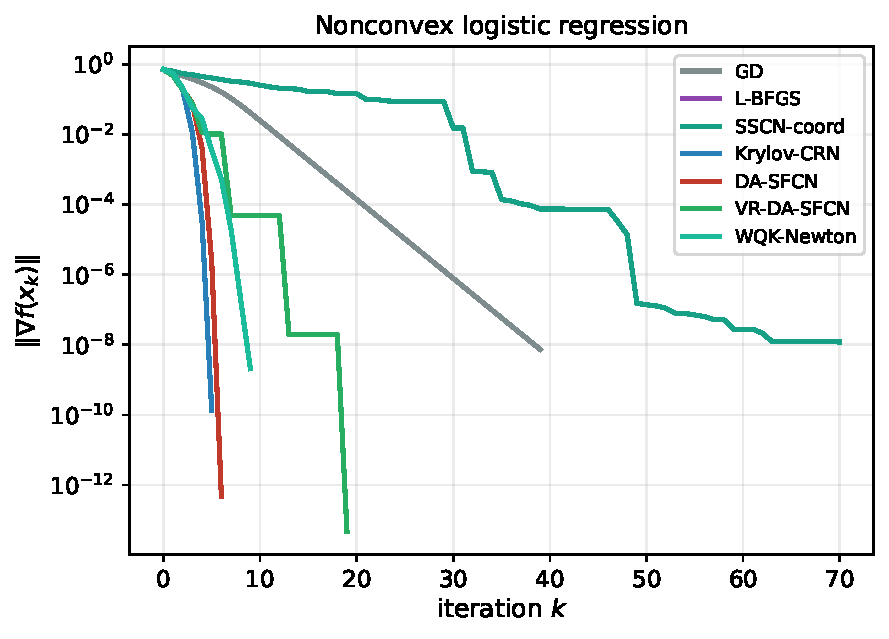
\includegraphics[width=0.48\textwidth]{fig_logistic.pdf}
\caption{معدل النجاح واللوجستي غير المحدب.}
\end{figure}
\begin{figure}[h]
\centering
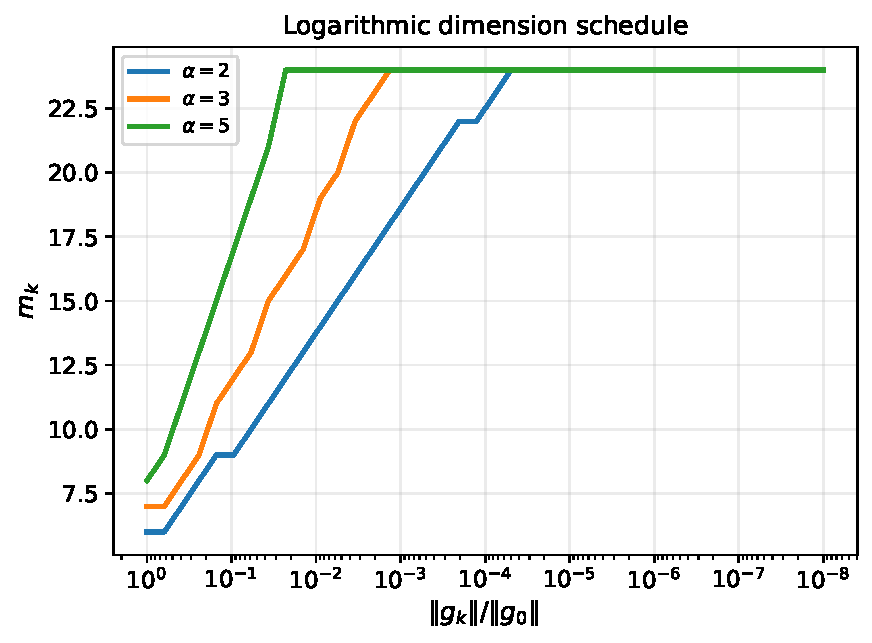
\includegraphics[width=0.48\textwidth]{fig_schedule_theory.pdf}
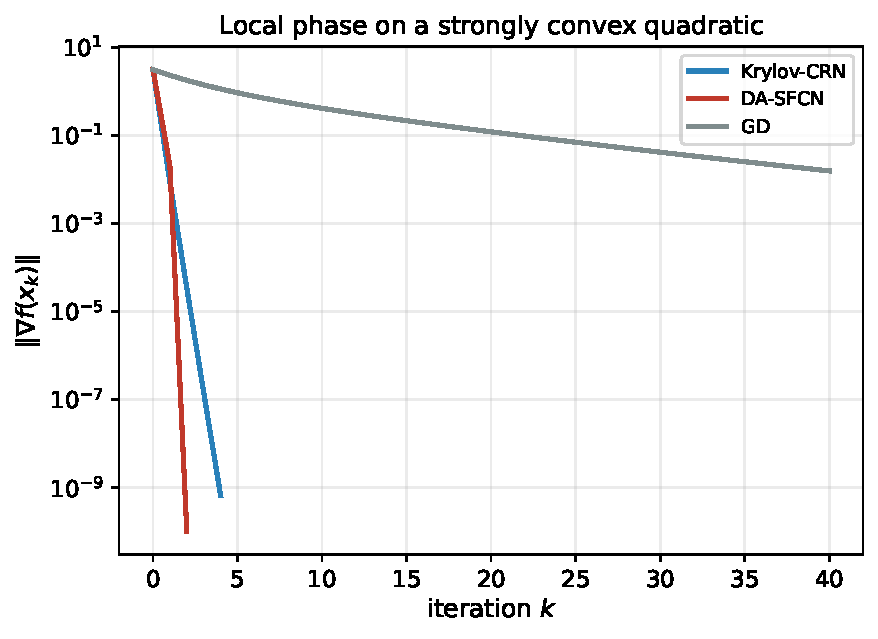
\includegraphics[width=0.48\textwidth]{fig_local.pdf}
\caption{الجدولة اللوغاريتمية والطور النيوتني المحلي.}
\end{figure}

على الرباعي $n=80$ نبلغ $f^\star\approx -89.58$ بـ $\|\nabla f\|\approx 1.5\times 10^{-7}$.
نجاح الهروب 100\%. اللوجستي: 6 تكرارات. الوعاء التربيعي: خطوتان إلى $10^{-10}$.

\section{الخاتمة}
هذه الخوارزمية أمّ العائلة: نواتها تُعاد في \textenglish{VR-DA-SFCN} و\textenglish{LK-Newton}
و\textenglish{WQK-Newton} و\textenglish{Fed-DA-SFCN} و\textenglish{SC-Newton}.

\begin{english}
\begin{thebibliography}{9}
\bibitem{nesterov2006} Nesterov, Polyak. \textit{Math.\ Program.}, 2006.
\bibitem{cartis2011} Cartis, Gould, Toint. \textit{Math.\ Program.}, 2011.
\bibitem{jiang2024} Jiang et al. \textit{AISTATS}, 2024.
\bibitem{dauphin2014} Dauphin et al. \textit{NeurIPS}, 2014.
\end{thebibliography}
\end{english}
\end{document}
